%-------------------------------------------------------------------------------
% LATEX TEMPLATE ARTIKEL
%-------------------------------------------------------------------------------
% Dit template is voor gebruik door studenten van de de bacheloropleiding 
% Informatica van de Universiteit van Amsterdam.
% Voor informatie over schrijfvaardigheden, zie 
%                               https://practicumav.nl/schrijven/index.html
%
%-------------------------------------------------------------------------------
%	PACKAGES EN DOCUMENT CONFIGURATIE
%-------------------------------------------------------------------------------

\documentclass{uva-inf-article}
\usepackage[english]{babel}
\usepackage{amsmath}
\usepackage{amssymb}
\usepackage{caption}
\usepackage{subcaption}

\usepackage[style=authoryear-comp]{biblatex}
\addbibresource{references.bib}

%-------------------------------------------------------------------------------
%	GEGEVENS VOOR IN DE TITEL, HEADER EN FOOTER
%-------------------------------------------------------------------------------

% Geef je artikel een logische titel die de inhoud dekt.
\title{Assignment 1: Estimating the area of the Mandelbrot set using Monte Carlo integration}

% Vul de naam van de opdracht in zoals gegeven door de docent en het type 
% opdracht, bijvoorbeeld 'technisch rapport' of 'essay'.
%\assignment{Naam van de opdracht}
%\assignmenttype{Type opdracht}

% Vul de volledige namen van alle auteurs in en de corresponderende UvAnetID's.
\authors{Alexander Künnen; Aaron De Clercq}
\uvanetids{UvAnetID 14101955; UvAnetID 14483610}

% Vul de naam van je tutor, begeleider (mentor), of docent / vakcoördinator in.
% Vermeld in ieder geval de naam van diegene die het artikel nakijkt!
\tutor{}
\mentor{}
\docent{Gábor Závodszky}

% Vul hier de naam van je tutorgroep, werkgroep, of practicumgroep in.
%\group{Naam van de groep}

% Vul de naam van de cursus in en de cursuscode, te vinden op o.a. DataNose.
\course{Stochastic simulations}
\courseid{}

% Dit is de datum die op het document komt te staan. Standaard is dat vandaag.
\date{\today}

%-------------------------------------------------------------------------------
%	VOORPAGINA 
%-------------------------------------------------------------------------------

\begin{document}
\maketitle

\justifying

%-------------------------------------------------------------------------------
%	INHOUDSOPGAVE EN ABSTRACT
%-------------------------------------------------------------------------------


%TC:ignore
%\tableofcontents
%\begin{abstract}
%\end{abstract}
%TC:endignore

%-------------------------------------------------------------------------------
%	INHOUD
%-------------------------------------------------------------------------------
% Hanteer bij benadering IMRAD: Introduction, Method, Results, Discussion.

\section{Introduction}

The Monte Carlo method is generally considered any approach that leads to a solution to a population-based problem by using a random sequence of numbers to represent a sample of the total population \parencite{halton1970}. It is a widely used method in the study of stochastic processes, like the behaviour of neutron chain reactions in fission devices \parencite{eckhardt1987} or the determination of efficiencies in gamma-ray detectors \parencite{raeside1976}.
The Monte Carlo method can also serve as a numerical integration technique to solve problems that are not necessarily stochastic. 
Compared to deterministic numerical integrators, such as the trapezoidal rule, the Monte Carlo integration method has a convergence rate independent of the dimensionality of the problem, indicating that it is a better technique for high-dimensional problems \parencite{james1980}.

Since the Monte Carlo integration method uses a random number generator, it is a non-deterministic method. Therefore, determining the quality as an estimator of the solution must be done statistically by looking at the variance.
Adding more sample points would reduce the variance and yield a better estimator, but this also increases the computational cost \parencite{james1980}.
Other techniques to reduce the variance, for example, stratified sampling and importance sampling, have been developed \parencite{james1980, kroese2012}.

To study the Monte Carlo integration method and the different variance reduction techniques in more detail, we will use them to estimate the area of the Mandelbrot set. The Mandelbrot set is the set of values in the complex plane for which the sequence,

\begin{equation}
    z_{n + 1} = z_n^2 + c
    \label{eq:mandelbrot}
\end{equation}

with $z_0$ equal to zero, remains bounded \parencite{ewing1992}.
Until now, there is no analytical expression to calculate the area of the Mandelbrot set, so the exact value of the area remains unknown \parencite{bittner2017}.
However, because the fraction of samples inside the Mandelbrot set is related to the area of the Mandelbrot set relative to the total sampling area, we can use the Monte Carlo integration technique to estimate the area.

In this process, there are two main approximations. The first one is the number of iterations for which we check if the sequence is bounded. For a value to be in the Mandelbrot set, equation \ref{eq:mandelbrot} should be bounded for every n, but we can only check this for a finite sequence. The second approximation is the number of sample points for which we check if the sequence is bounded. A particularly interesting question is how the estimate of the area changes if we vary the number of iterations or the number of sampling points.

Additionally, we can look at the effect of using stratified sampling techniques on the convergence rate. With Latin hypercube sampling \parencite{wei1996} and orthogonal sampling, the idea is to subdivide the total sampling area into subareas to get a more homogeneous sampling strategy. As these are known ways to reduce the variance, we can assume that the estimate of the area of the Mandelbrot set would improve compared to pure random sampling.

In the final part, we will test if a combination of stratified and importance sampling can further improve the convergence rate.

\section{Theory}
    
    FIFO\\
    First in First Out scheduling refers to a method in computational sciences in which a queueing 
    process is used to store a number of tasks which are then performed in order of arrival 
    at that queue. The assumption being that there is a specific order for the tasks to arrive at
    the queue.\\
    
    https://projecteuclid.org/journals/annals-of-mathematical-statistics/volume-24/issue-3/Stochastic-Processes-Occurring-in-the-Theory-of-Queues-and-their/10.1214/aoms/1177728975.full\\


    Kendalls Notation\\
    Kendalls Notation as used in the 1953 Paper of Kendall consist of 3 entries in the form of X/Y/n.
    X denotes the distribution of input signals/ arrivals of tasks in the queue, Y the distribution of 
    server-worktime or the amount of time necessary to perform a task and n being the amount of servernodes 
    taking on tasks.
    Kendall noted several distributions in their paper-
    For the following A(u) is probability of a given task arriving after a given time u.\\
    D;Deterministic:
\begin{equation}\label{eq:determ}
	\begin{split}
		\text {Each task arrives at a given time($\mu$)}\\
        A(u) = \text { if  }u<\mu : 0 \text{ else : } 1
    \end{split}
	\end{equation}
    M;"random" or Poisson distributed
    \begin{equation}\label{eq:poisson}
    A(u) = 1-e^{-u/\mu}
	\end{equation}
    $E_k$; Erlangian
    \begin{equation}\label{eq:erlang}
        E_k \text { (Erlangian): } d A(u) \equiv \frac{(k / a)^k}{\Gamma(k)} e^{-k u / a} u^{k-1} d u\\
	\end{equation}
    G/GI; No assumption is taken for the distribution\\
    
    One example is the M/M/n $(n \in \mathbb{N})$ queueing simulation(poisson distributed Arrivals and server worktime with n servers). 
    which we will focus on.
    
  
\section{Methodology}

\subsection{Varying the number of iterations and sample points}

We can study the effect of changing the number of iterations by keeping all the other parameters in the calculation of the area constant. First, we generate 1000 random sample points, uniformly distributed in the total sampling area (${[-2,2] +[-2i,2i]}$).
Using these sample points, we calculate the estimated area of the Mandelbrot set with the number of iterations varying from $2^1$ to $2^{15}$.

For the effect of changing the number of sample points, we set the number of iterations fixed to 500 and calculate the average estimated area over 100 runs.
We do this calculation with the number of sample points varying from $2^3$ to $2^{12}$.

\subsection{Effect of stratified sampling}

To see whether the stratified sampling methods, Latin hypercube sampling and orthogonal sampling reduce the variance of the estimated area compared to uniform sampling, we run 100 calculations using each sampling method.
During these calculations, we set the number of iterations equal to 500 and we also perform these calculations using different numbers of sample points. That way we can check if the difference in the variance between the sampling methods depends on the number of sampling points.

To test if the difference between the average estimated area with different sampling methods is significant, we can use Welch's t-test. For the difference in the variance, we will use an F-test to see if this difference is significant.

\subsection{Strategic sampling to improve the convergence rate}

We used strategic sampling of the area $\mathbb{C} \supset \{[-2,2] +[-2i,2i]\}$(see Mandelbrot set in theory part for reason) to calculate the area of the Mandelbrot set and compared the results to 
the orthogonal/Latin hypercube sampled Monte Carlo Method in the same area.
The basic idea was to focus more on the areas where it cannot a-priory be inferred whether the samples 
will belong to the Mandelbrot set or not.
For this purpose we devised a sub-spacing algorithm, taking into account the first $x_k = x_{k-1}+ 128 * (2^k)$ 
samples, with k being the iterator for that specific cycle, and determining if a specific subspace contains only samples that are in the set or out. The samples inside each subarea were generated through Latin hypercube sampling. The area was divided into $sa_k = 16*(4^(k/2))$(with k/2 being rounded down) sub-spaces with a corresponding value for sample probability and test-iterations in the subarea. 
In that case, future samples will be less likely taken out of that area. This is supposed to increase the
precision of the result in the areas where there are both samples in the Mandelbrot set and outside.
The number of samples in a subspace is set deterministic by the total number of samples required and the sample probability of that subspace.
In each cycle, we increased the number of samples $x_k$ and in the strategic sampling version the number of subareas $sa_k$. 
The resulting subareas will be added to the total area by their relative size. 
\\
We ran 100 experiments for the Monte Carlo method with orthogonal sampling, Latin hypercube sampling and the strategic sampling method, with 
6 cycles each. Resulting in the following configurations across the 6 Cycles.


%\begin{tabular}{t | 1 | 2 | 3 | 4 | 5 | 6}
%\textbf{Cycle }&1&2 &3 &4&5&6\\
%\hline
%\textbf{Samples per cycle(L.-H./Orth.)}&256&784&1849&3844&8100&16129\\
%\textbf{Samples per cycle(Strat.)}&256&768&1792&3840&7936&16128\\
%\textbf{Subdivisions(L.-H./Orth.)}&1&1&1&1&1&1\\
%\textbf{Subdivisions(Strat)}&16&64&64&256&256&1048\\
%\end{tabular}
The amount of samples used for the comparison(Latin hypercube/Orthogonal sampling) was slightly different for practical reasons, but chosen to be as close as possible to the samples used in strategic sampling..
After running the 100 experiments with these parameters, we get an array of resulting area estimations.
The statistical tests mentioned in the theory part were performed on these data points, resulting in hypothesis tests to infer whether we could reliably tell if the two methods show different or improved convergence rates in both accuracy and precision.\\
The following sequence of graphs shows how samples are selected in each cycle.\\

\begin{figure}[h]
    \centering
    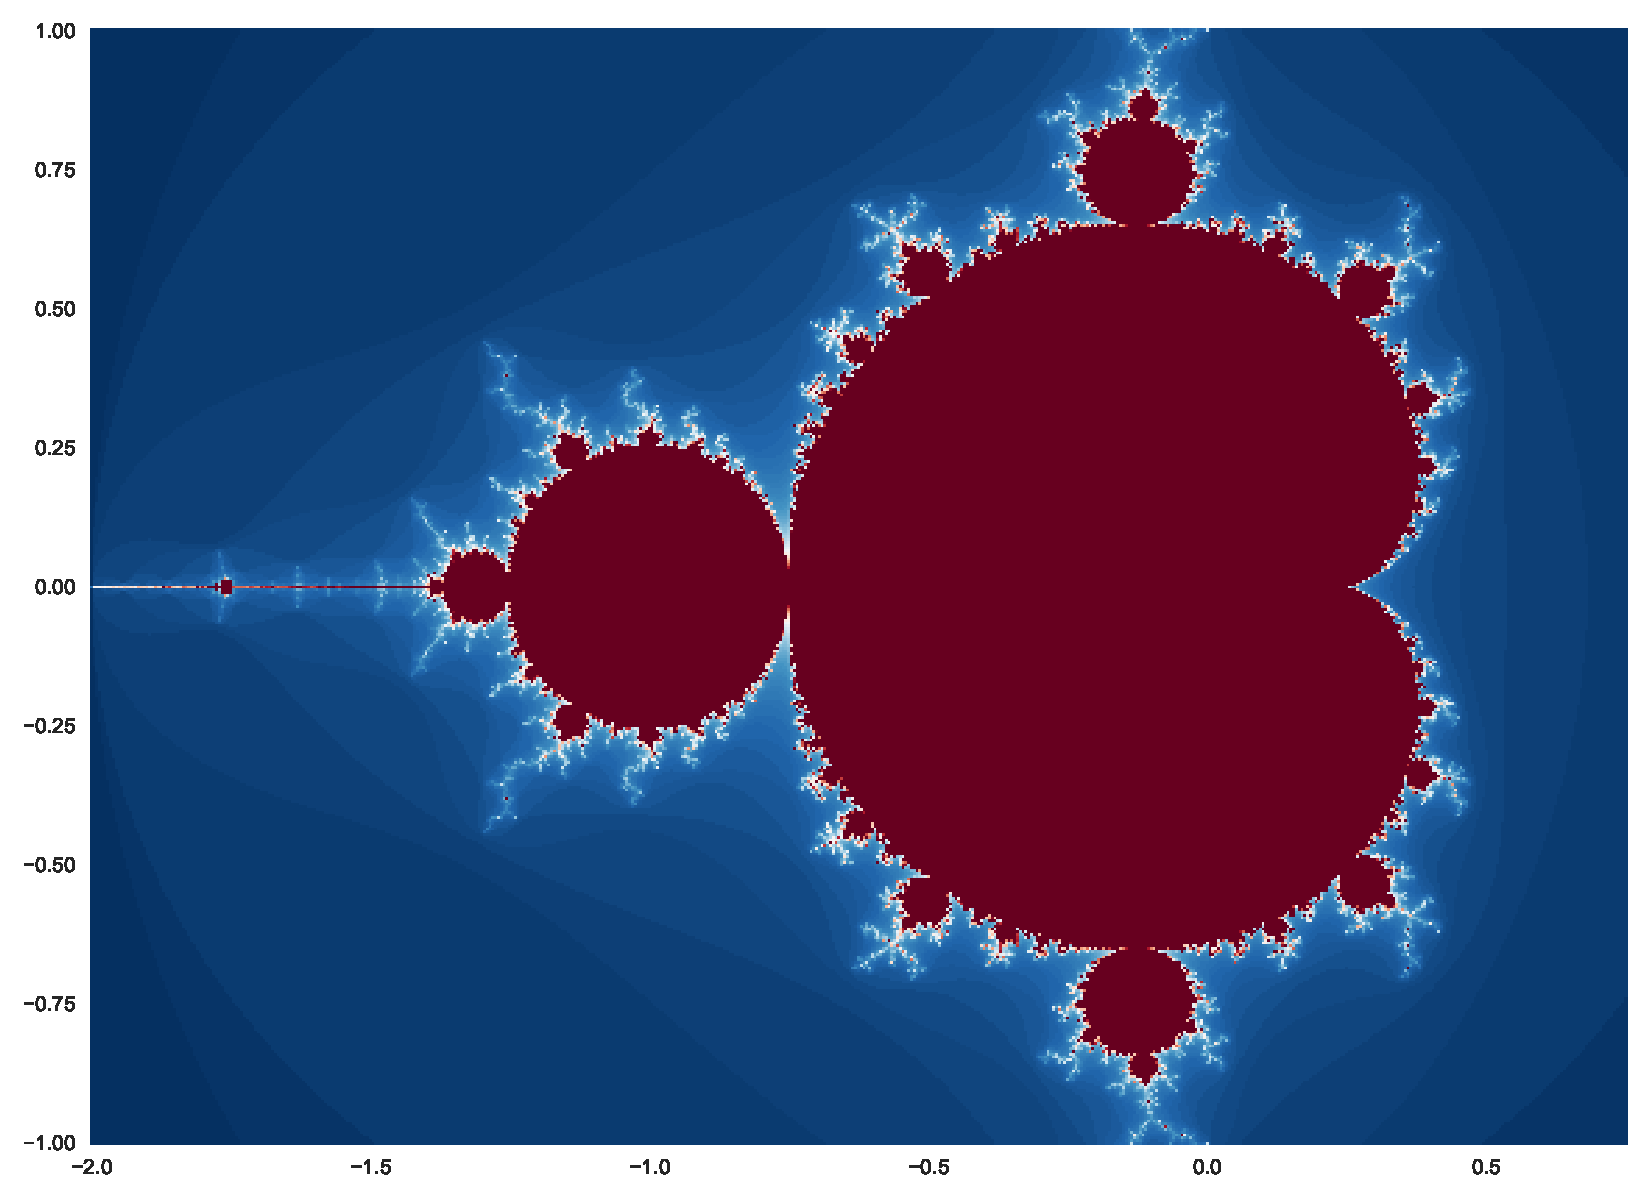
\includegraphics[width=.85\textwidth]{fractal.pdf}
    \caption{The samples taken in Strategic sampling while progressing through cycles.}
    \label{fig:samples_ss}
\end{figure}


\section{Results and discussion}
\subsection{Varying the number or iterations and sample points}

The left graph in figure \ref{fig:var_i_s} shows the estimated area of the Mandelbrot set as a function of the number of iterations, where the area is corrected with respect to the estimated area for the maximal number of iterations.
At low iterations, we see that the area of the Mandelbrot set is highly overestimated.
This is because many sample points are considered inside the Mandelbrot set because the value has a magnitude below 2 during the first few iterations of the sequence.
Increasing the number of iterations will lead to a reduction of the estimated area because values for which it takes a while before the sequence starts to diverge are correctly assigned as outside the set. 
This means that increasing the number of iterations will lead to higher accuracy of the estimation.\\

In the right graph of figure \ref{fig:var_i_s}, we keep the number of iterations constant and plot the average estimated area over 100 simulations as a function of the number of sample points.
The edges of the coloured area represent the average area $\pm$ the sample variance.
When using very few sample points, the average area is slightly underestimated because the sampling area is much bigger than the Mandelbrot area.
Increasing the number of sample points leads to a significant reduction in the variance between different simulations.

\begin{figure}[h]
    \centering
   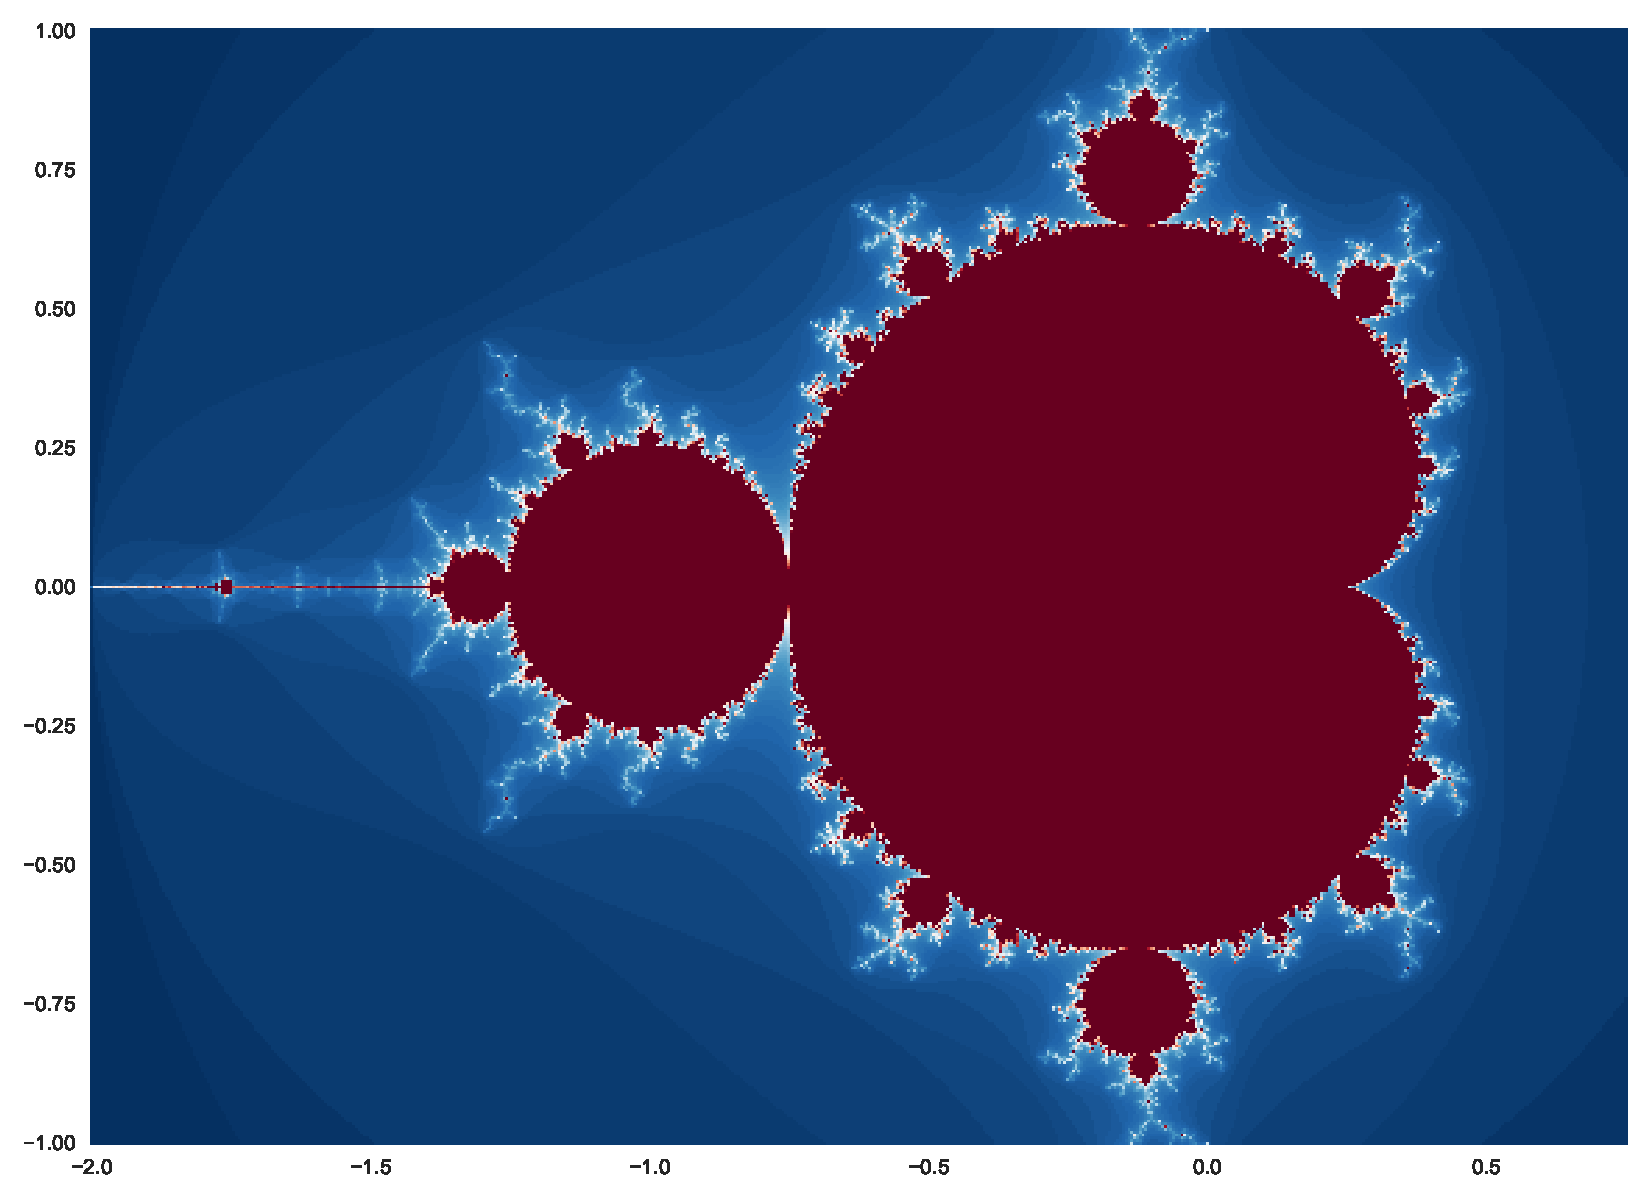
\includegraphics[width=.85\textwidth]{fractal.pdf}
    \caption{Estimate of the area of the Mandelbrot set as a function of the number of iterations and samples.}
    \label{fig:var_i_s}
\end{figure}

\subsection{Effect of stratified sampling}

Figure \ref{fig:stratified} shows the average estimated area and the sample variance as a function of the number of sampling points.
When using a low number of sampling points, the Latin hypercube sampling method will have a higher estimated area compared to Latin hypercube and uniform sampling. Looking at the left graph \ref{fig:stratified_stats}, the difference in the average area between uniform and Latin hypercube / Latin hypercube and orthogonal sampling is only significant for the lowest number of sampling points.
Increasing the number of sampling points shows that all three sampling methods converge towards the same estimated area.\\

In the right graph of figure \ref{fig:stratified}, the sample variance is plotted as a function of the number of sampling points. The sample variance is clearly the highest for uniform sampling and orthogonal sampling results in the lowest variance. The results of an F-test, shown in the right graph of figure \ref{fig:stratified_stats}, indicate that the difference in the variance is significant for all the number of sampling points.
This indicates that orthogonal sampling is the better technique compared to Latin hypercube sampling to improve the variance reduction.

\begin{figure}[h]
    \centering
    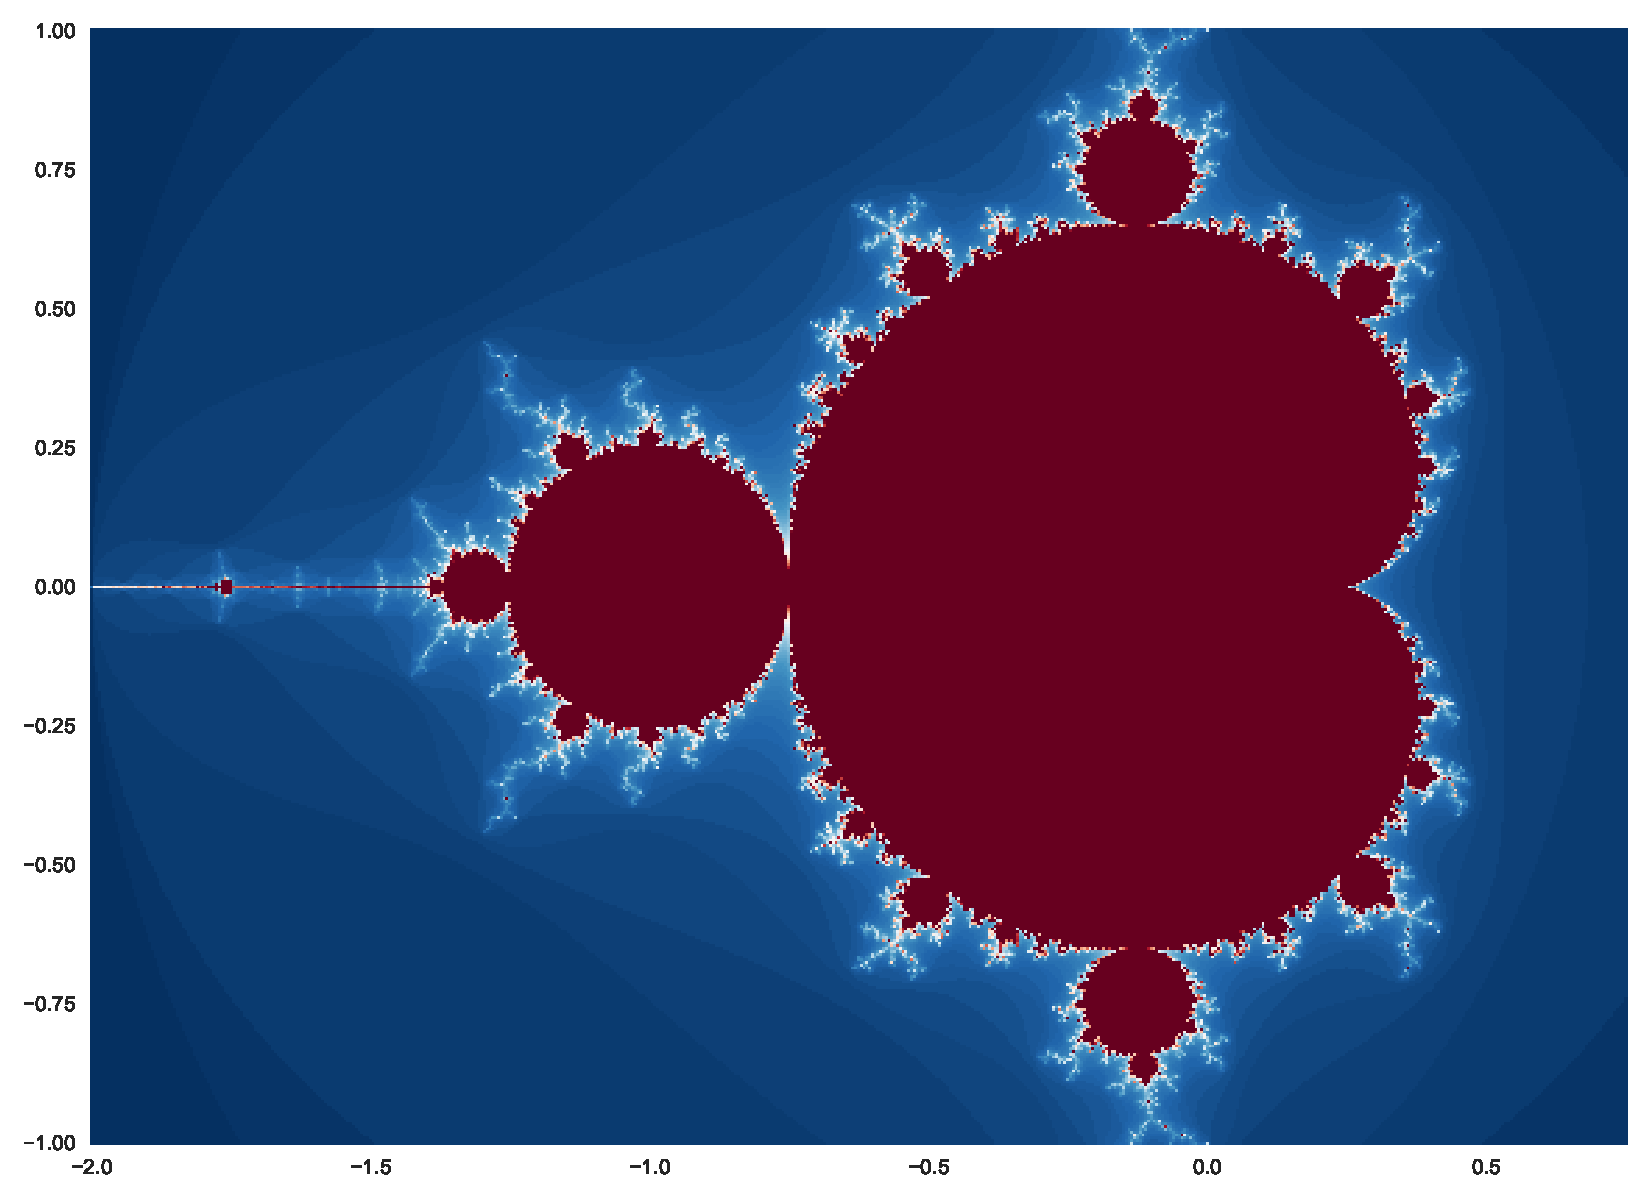
\includegraphics[width=.85\textwidth]{fractal.pdf}
    \caption{Estimate of the area of the Mandelbrot set using different sampling strategies.}
    \label{fig:stratified}
\end{figure}

\begin{figure}[h]
    \centering
   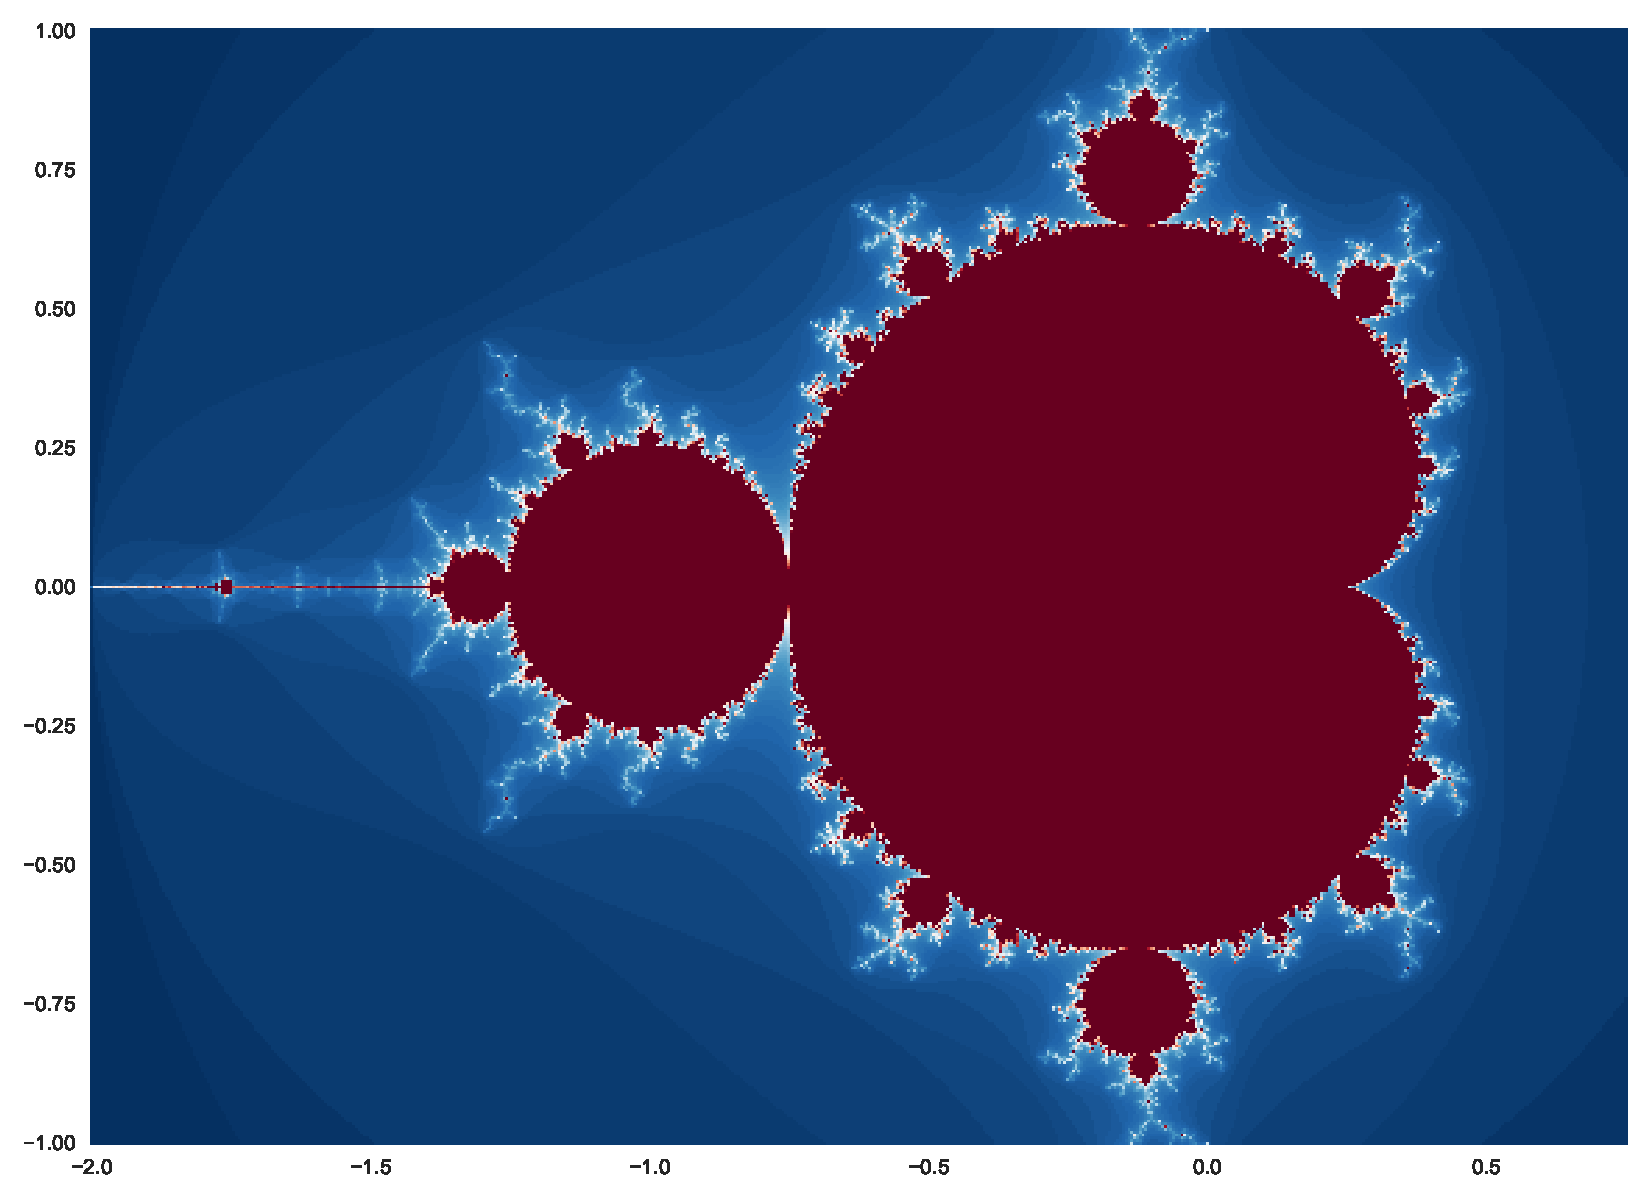
\includegraphics[width=.85\textwidth]{fractal.pdf}
    \caption{Left: p-values of a Welch t-test as a function of the number of sampling points. Right: F-values as a function of the number of sampling points.}
    \label{fig:stratified_stats}
\end{figure}


\subsection{Strategic sampling to improve the convergence rate}
We compared the results of the Strategic sampling method against Latin hypercube/orthogonal sampling to determine whether the mean or variance is impacted by the choice of method. The exact Statistical tests were discussed in the Theory part. The Null Hypothesis was described as the results being virtually similar.

\subsubsection{Accuracy}

To determine if the accuracy of the results is affected we compared the means in figure \ref{fig:c_mean} showing the overlap in confidence intervals. The confidence intervals were created by adding the standard deviation of the sample group to the mean in that cycle. For orthogonal sampling, the confidence intervals overlap neatly whereas for Latin hypercube sampling the confidence intervals show distinct areas. In each case, the averages of the samples lie inside the confidence intervals of both methods.\\

\begin{figure}[h!]
  \centering
 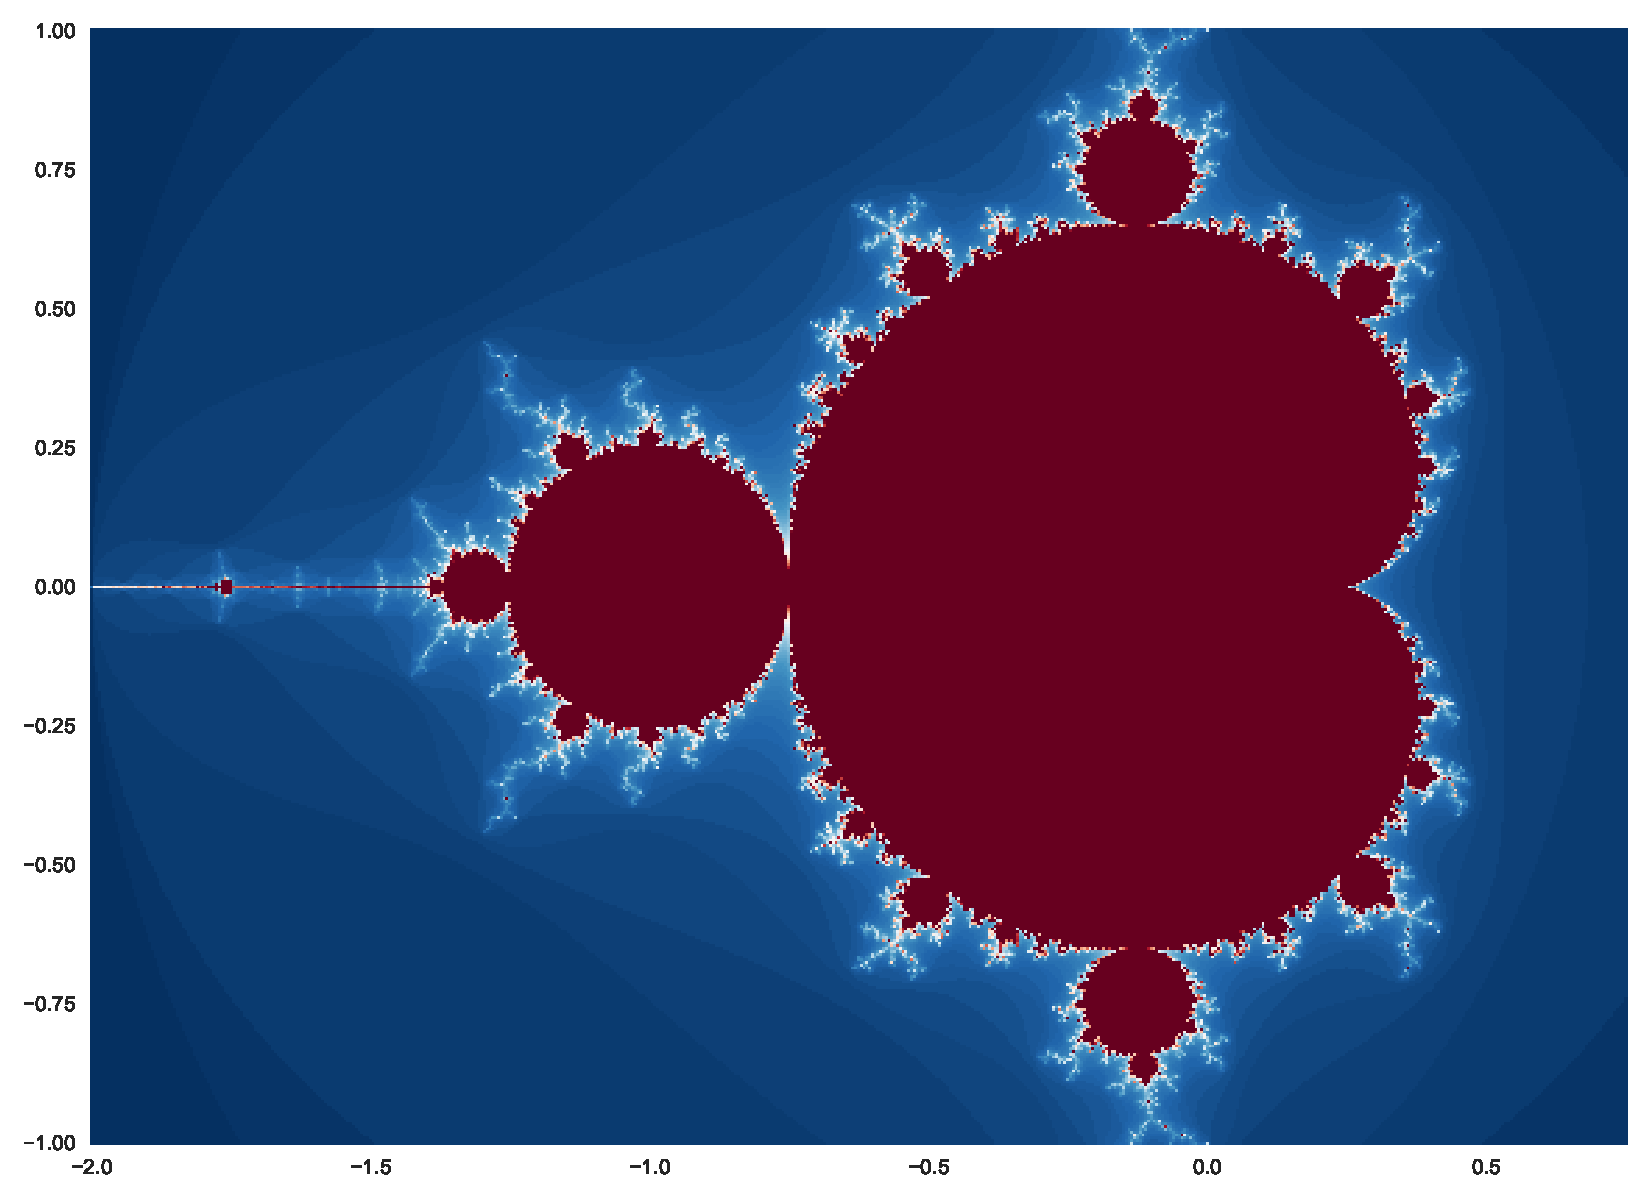
\includegraphics[width=.85\textwidth]{fractal.pdf}
  \caption{Mean comparison with 1-sigma confidence intervals using Latin hypercube(right) and orthogonal sampling(left) when compared with Strategic Sampling. The dashed green Line represents the measured value for the Mandelbrot set area from \parencite{mitchell2001}}
  \label{fig:c_mean}
\end{figure}
  

The Welch's T-test, shown in figure \ref{fig:welch_t}, compares the Welch's T-value in each cycle against the required critical value, to reject the null hypothesis. The orthogonal sampling method shows one distinct value in all the cycles, otherwise, the critical value is not surpassed.\\
\begin{figure}[h!]
  \centering
  %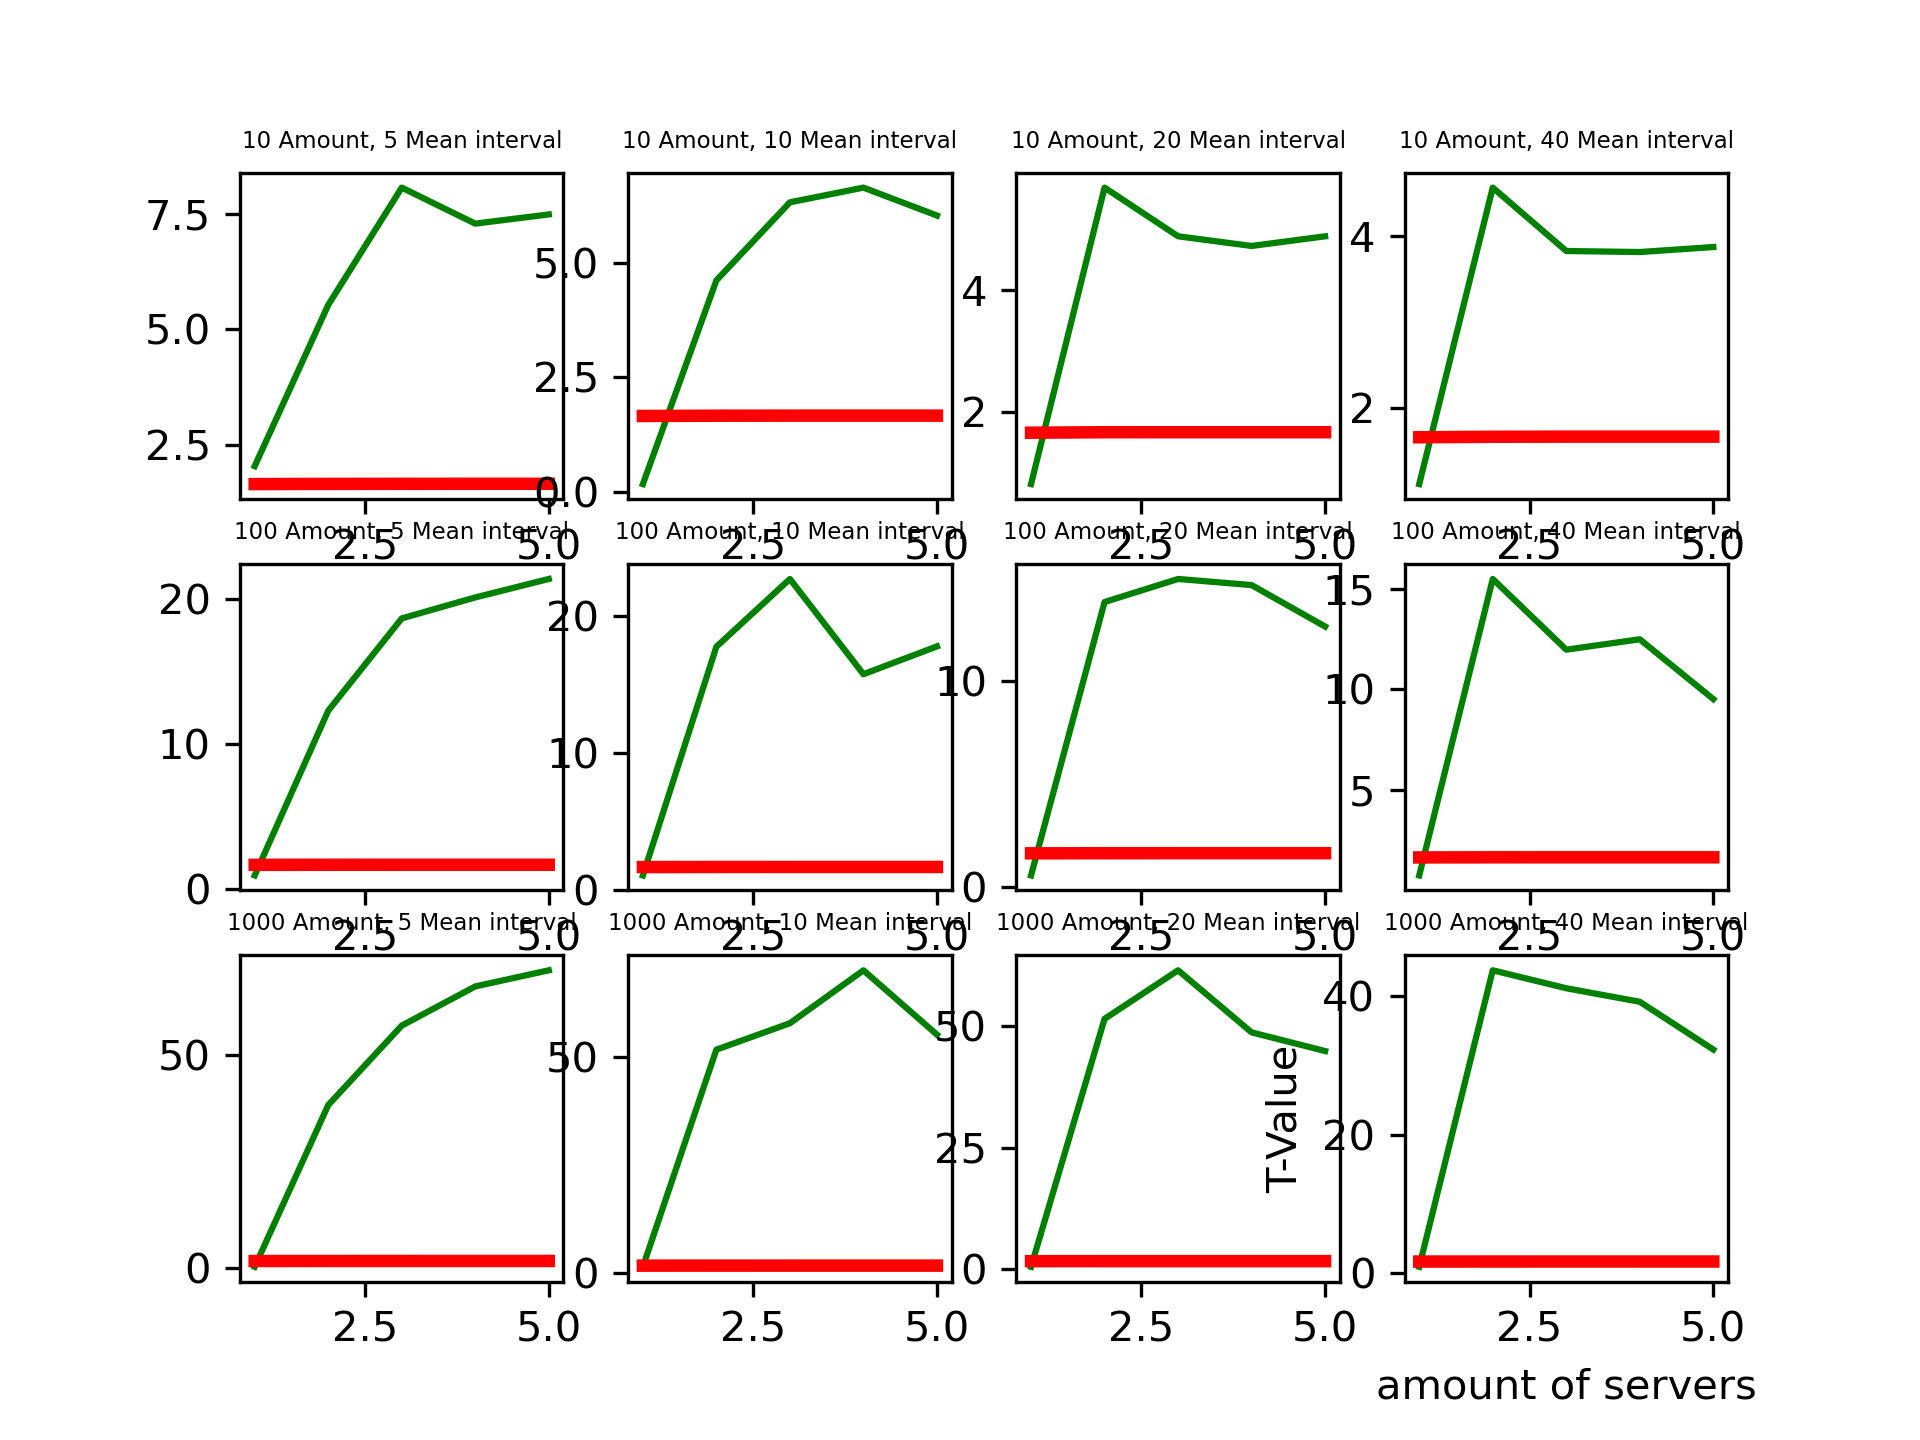
\includegraphics[scale=0.4]{welch_t_test_noTitle.png}
  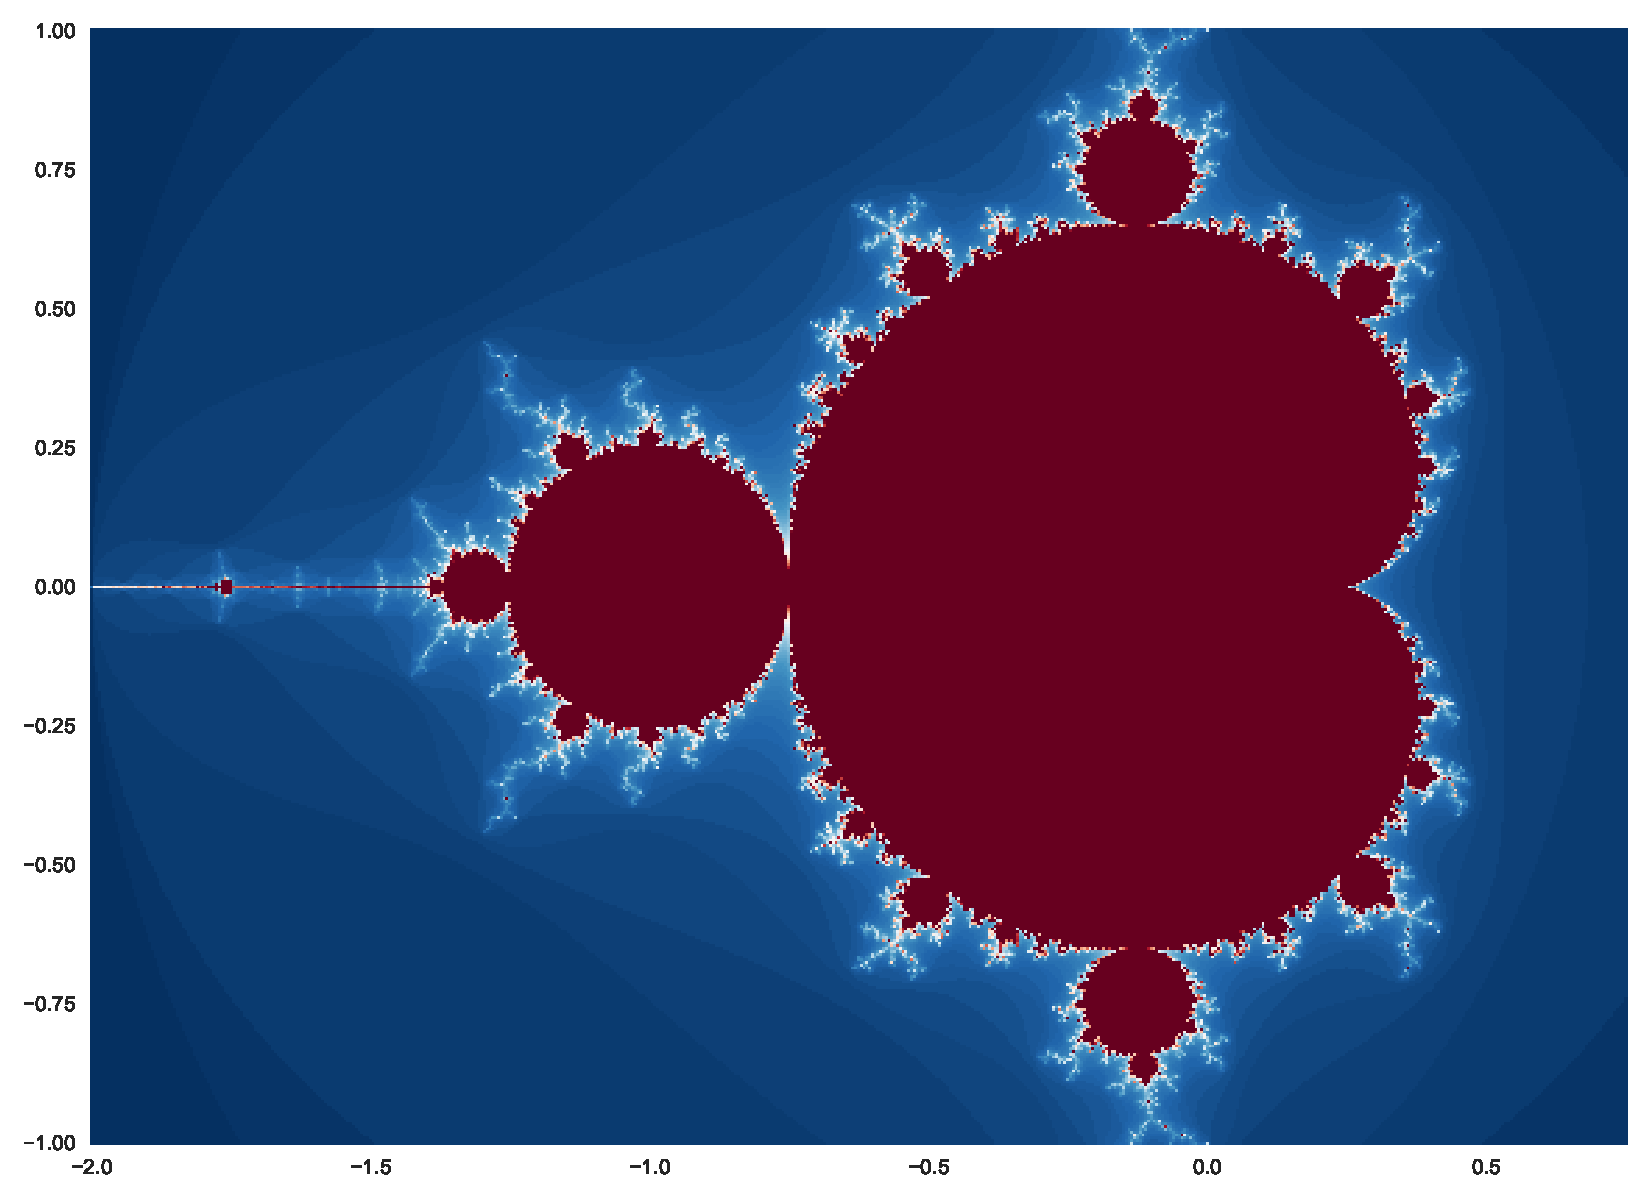
\includegraphics[width=.85\textwidth]{fractal.pdf}
  \caption{Welch's T-test comparing the mean distributions for Strategic sampling with Latin hypercube(right) and orthogonal sampling(left) with the critical T-value(red) with significance level 0.05}
  \label{fig:welch_t}
\end{figure}

The T test shows that the mean values are not separate for the different values. The one outlier in figure \ref{fig:welch_t} can be attributed to randomness since the experiment is repeated for several cycles and subsequent values are not affected. This suggests our method does not improve the accuracy of the results.


\subsubsection{Precision}

To find out if the precision of the result is affected by the method we compared the variances  (figure \ref{fig:log_var}) in the sample groups and performed a F-test (figure \ref{fig:f_test}) which was compared against the corresponding critical F-value for significance.
In figure \ref{fig:log_var}, the variance of the Latin hypercube sampling method was constantly higher than the Strategic sampling method, whereas the variance of the orthogonal sampling method had very similar results to our applied method.\\

\begin{figure}[h!]
  %\includegraphics[scale=0.4]{l}
  \centering
 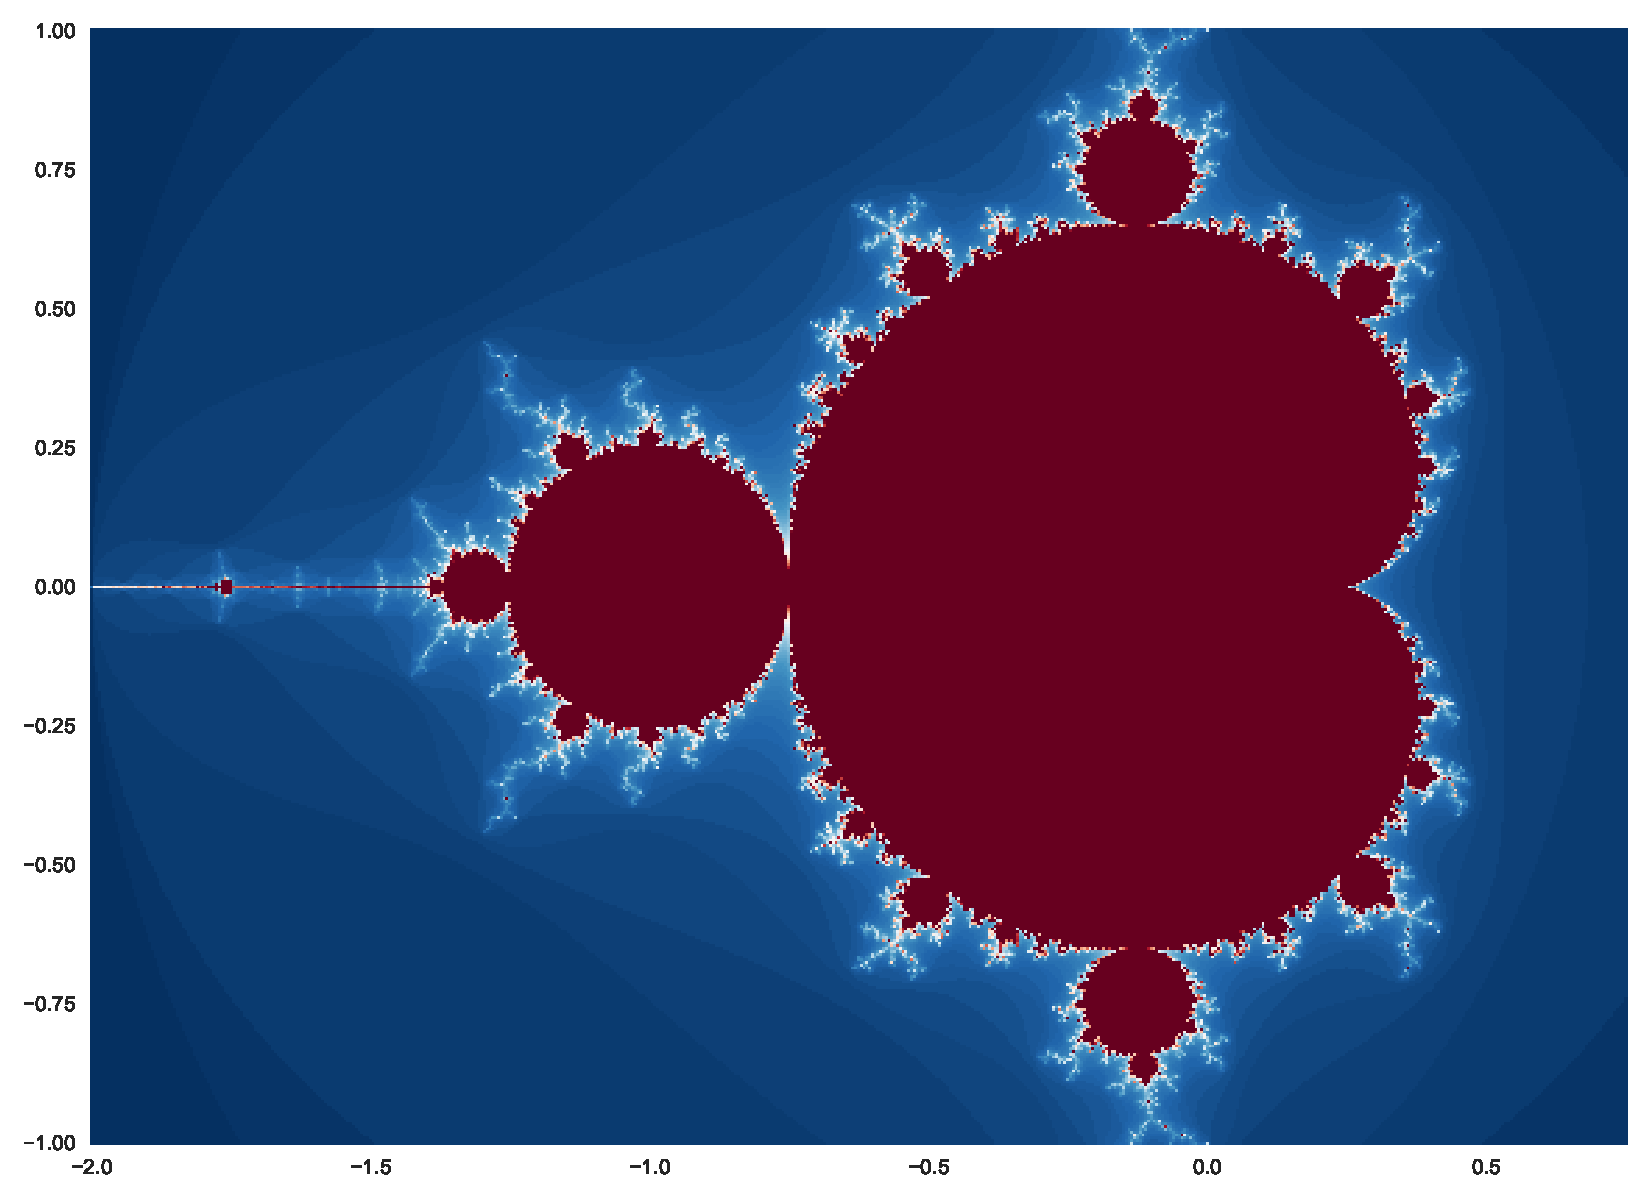
\includegraphics[width=.85\textwidth]{fractal.pdf}
  \caption{Difference in variance in between Strategic sampling(red) and Latin hypercube(yellow)/ orthogonal sampling(blue) as shown on a logarithmic scale}
  \label{fig:log_var}
\end{figure}

In the F-test (figure \ref{fig:f_test}), the F-value for the Latin hypercube sampling comparison is always above the critical value.
The orthogonal Sampling comparison lies close to the critical value for the most part but shows two occasions clearly surpassing the value in a cycle.\\

\begin{figure}[h!]
  \centering
  %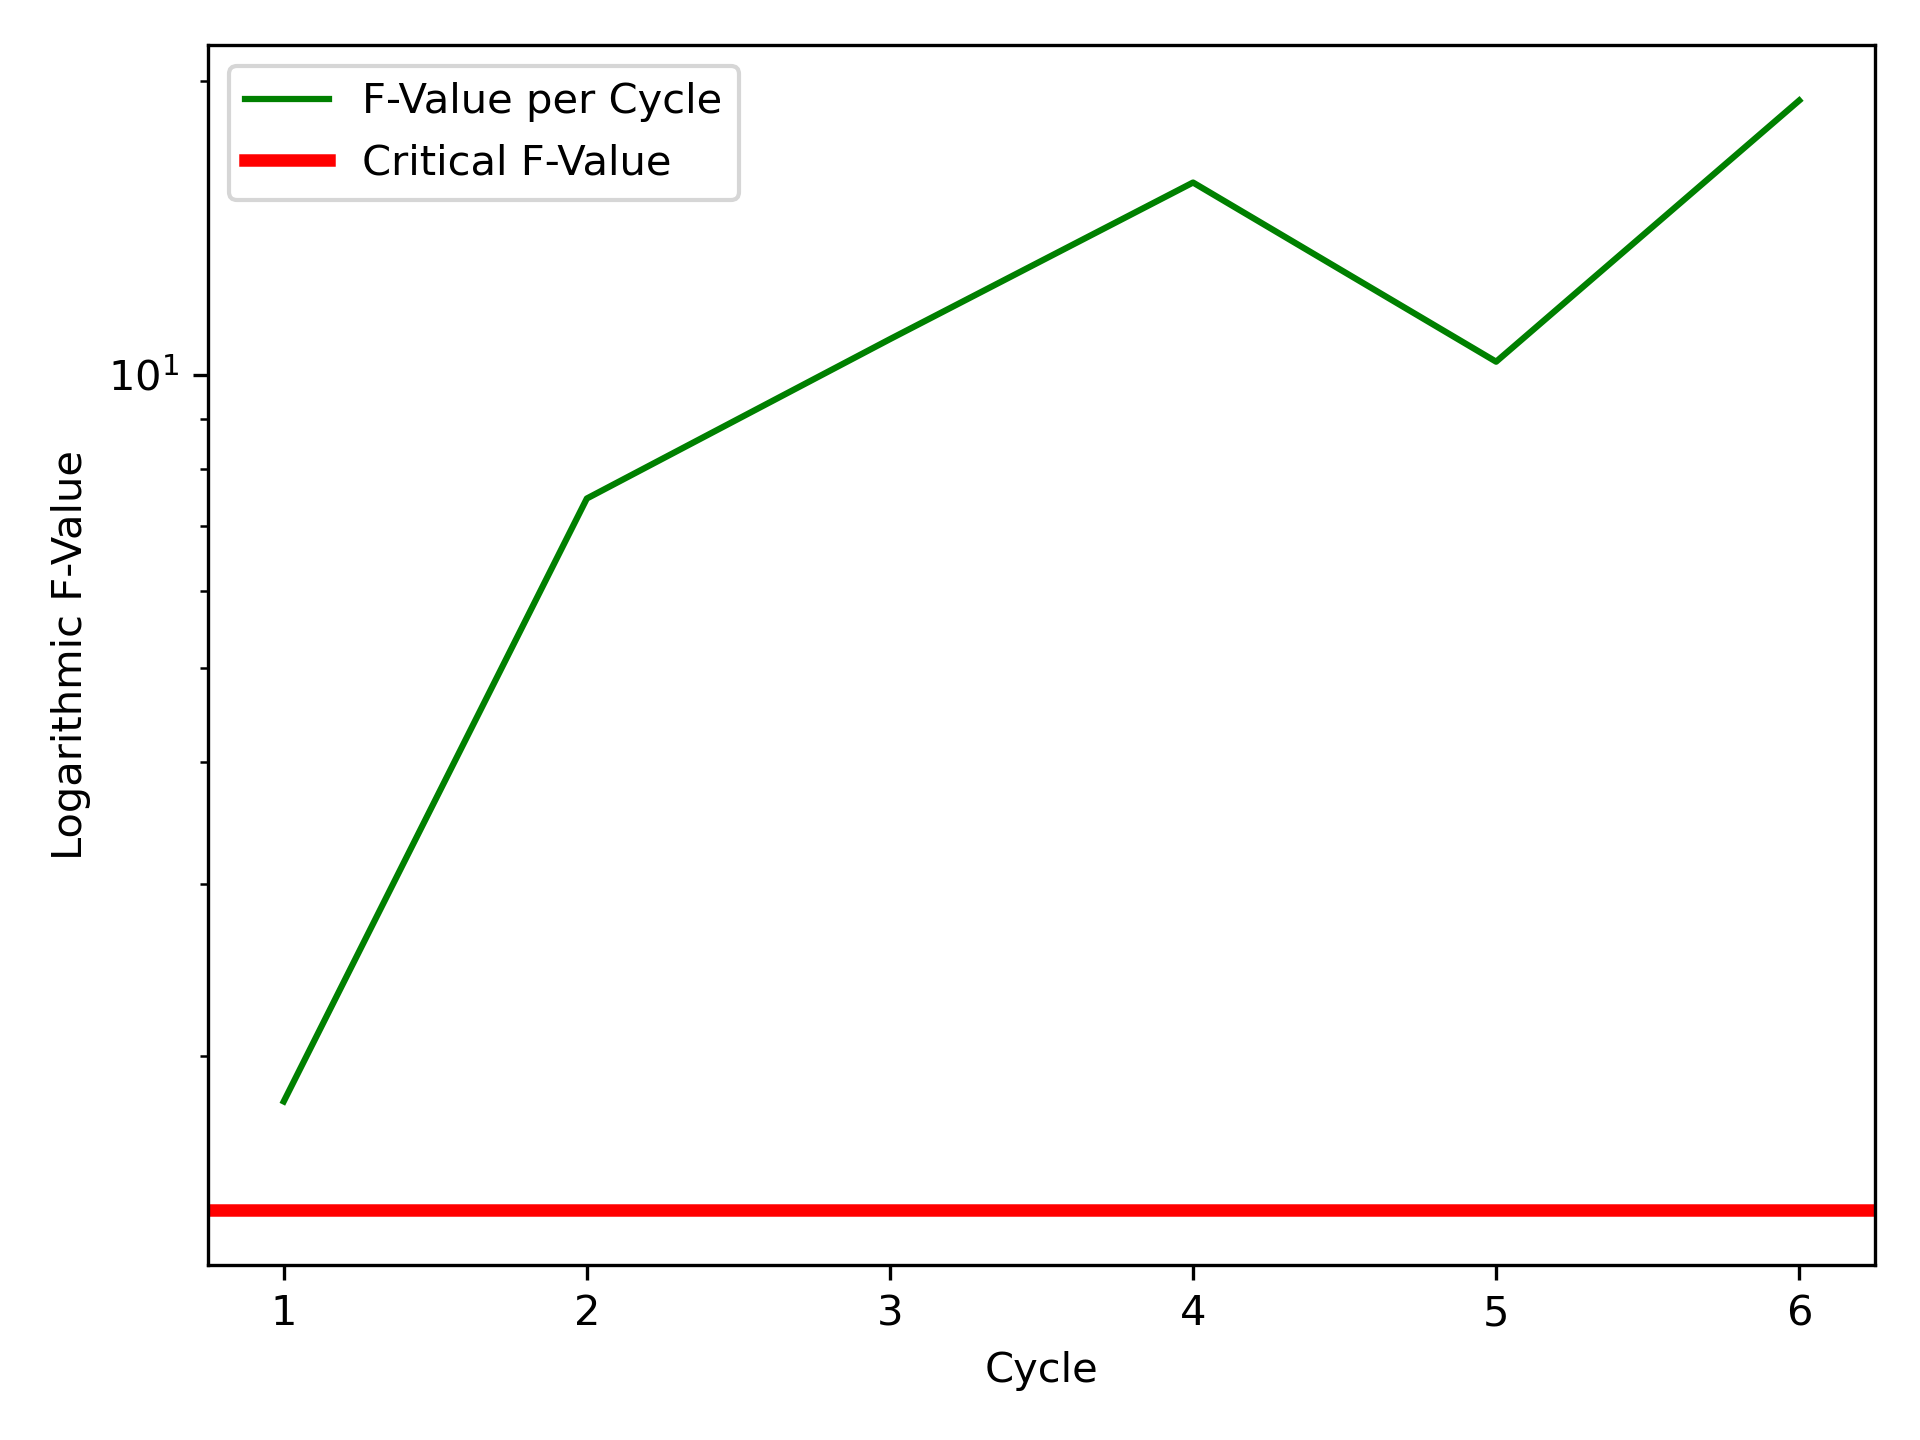
\includegraphics[scale=0.4]{one_sided_f_test_noTitle.png}
  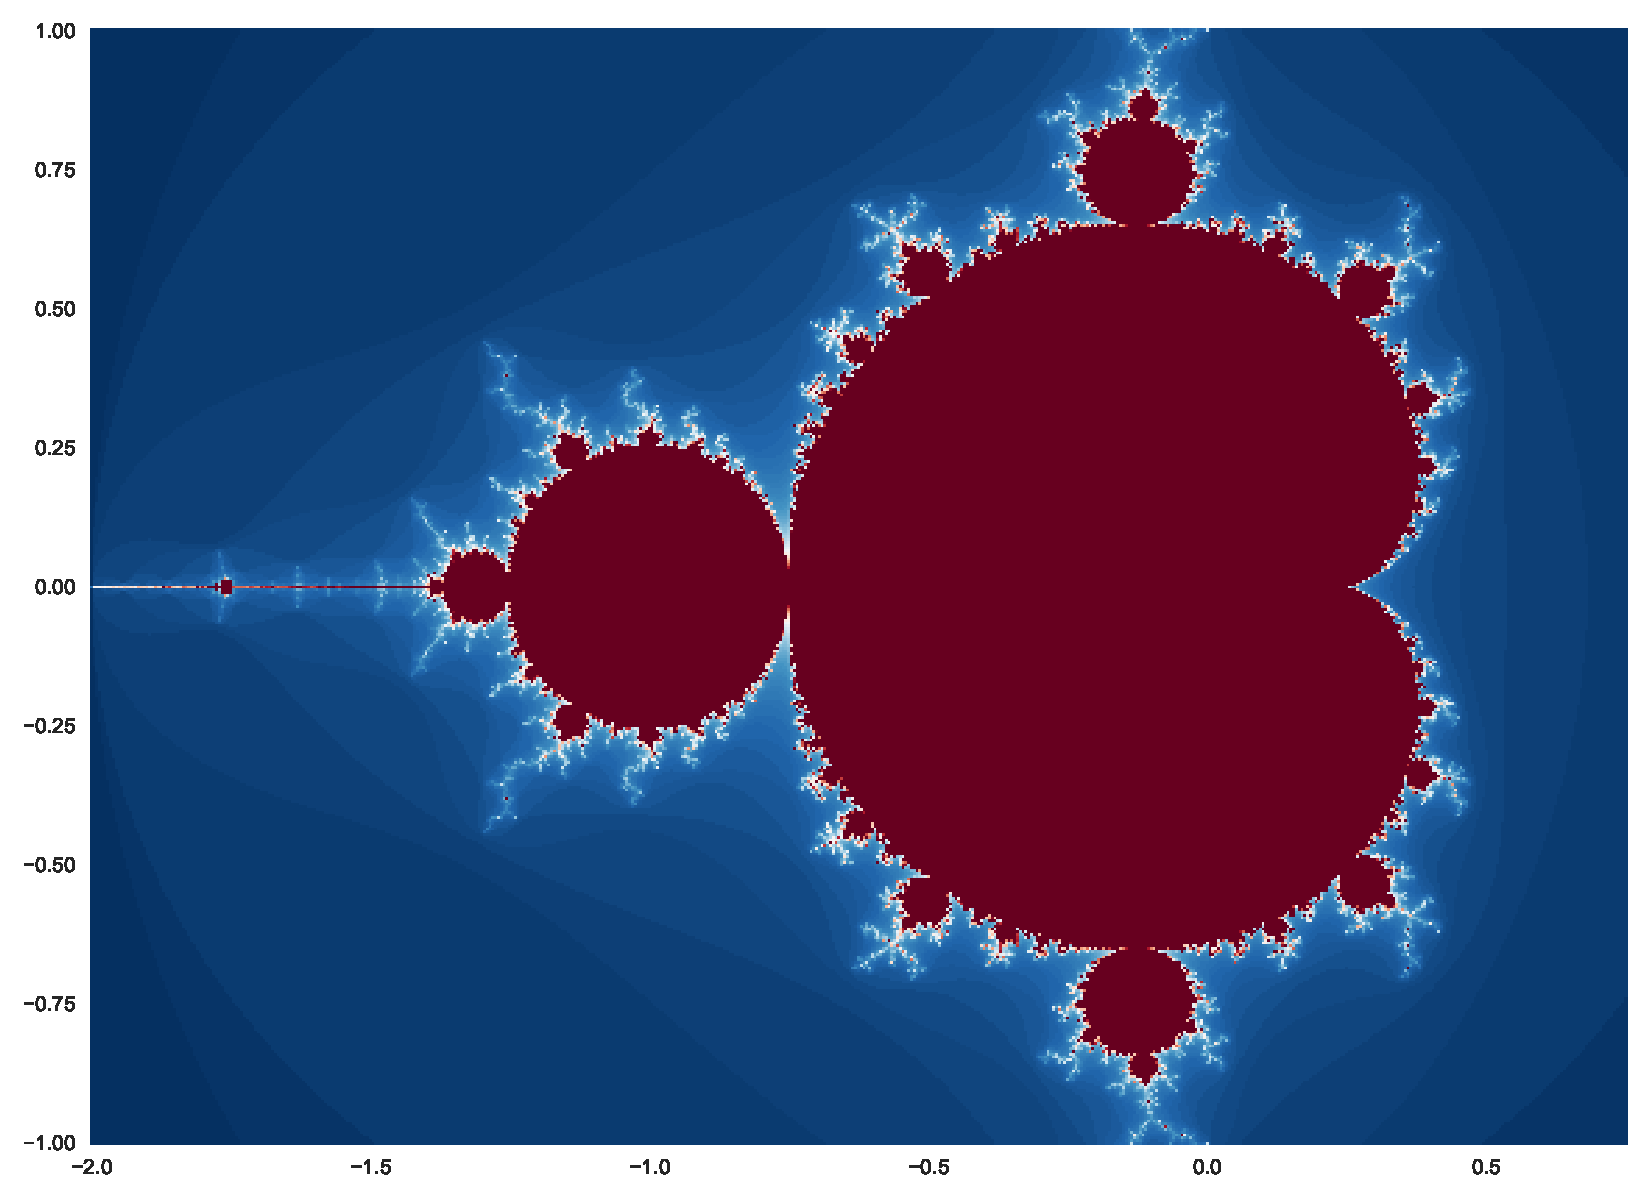
\includegraphics[width=.85\textwidth]{fractal.pdf}
  \caption{F-test comparing the variance distributions for Strategic sampling with Latin hypercube(right) and orthogonal sampling(left) with the critical F-value(red) with significance level 0.05 as shown on a logarithmic scale}
  \label{fig:f_test}
\end{figure}

This shows that our method improved the variance and therefore the precision compared to Latin hypercube sampling since the F-test suggests two differing variances while the variance is higher for Latin hypercube sampling (figure \ref{fig:log_var}). On the other hand, orthogonal sampling still converges either similarly fast or even faster than Strategic sampling as suggested by their respective plots in figure \ref{fig:log_var} and \ref{fig:f_test}.


\newpage
\section{Conclusions}
In conclusion, we were able to show that increasing the number of iterations to check for divergence in the Mandelbrot set improved the overall accuracy of the result, specifically reduced the resulting area, while the number of samples used for calculating the result in a Monte Carlo simulation increased the precision/ decreased the variance in the resulting area estimations.\\
Also when comparing sampling methods uniform, Latin hypercube and orthogonal we found no evidence suggesting they affect the overall accuracy but found the Latin hypercube sampling method to improve the precision compared to uniform sampling and orthogonal sampling to improve the precision compared to Latin hypercube sampling.\\
Furthermore, we improved the precision of the Monte Carlo Method estimating the area of the Mandelbrot set using Strategic sampling compared to Latin hypercube sampling which it was based on, but could not affect the accuracy of the result similar to previous results.
The orthogonal Sampling Method on the other hand was able either outperform or contest the Strategic Sampling approach by itself. \\
Future Precision improvements seem plausible when applying orthogonal sampling to the sampling methods in the subareas instead of Latin hypercube sampling. Due to time constraints, this approach could not be investigated in this report.

%-------------------------------------------------------------------------------
%	REFERENTIES
%-------------------------------------------------------------------------------
\clearpage
\printbibliography

%-------------------------------------------------------------------------------
%	BIJLAGEN 
%-------------------------------------------------------------------------------

%TC:ignore
%\appendix 
%\section{Bijlage {\LaTeX} code}
%Bijgevoegd zijn de \textattachfile{main.tex}{code} en 
%\textattachfile{references.bib}{bibliografie}.
%TC:endignore

%-------------------------------------------------------------------------------
\end{document}